
\subsection{Diseño de la interfaz de usuario}
\label{sec:diseno-ux-diseno}
La interfaz de usuario es la parte de la aplicación que permite la interacción con el sistema. En \textit{Ott}, 
se encarga de mostrar la información al usuario y permitirle navegar y utilizar las funcionalidades. 
Es esencial que la interfaz sea clara, sencilla e intuitiva, para garantizar una experiencia de uso eficiente.

El diseño inicial no partió de un esquema definitivo, ya que debía adaptarse a las necesidades de los clientes. 
Se desarrolló una interfaz base que facilitara la incorporación de nuevas funcionalidades y la personalización 
según los requisitos de cada cliente.

\begin{figure}[H]
    \centering
    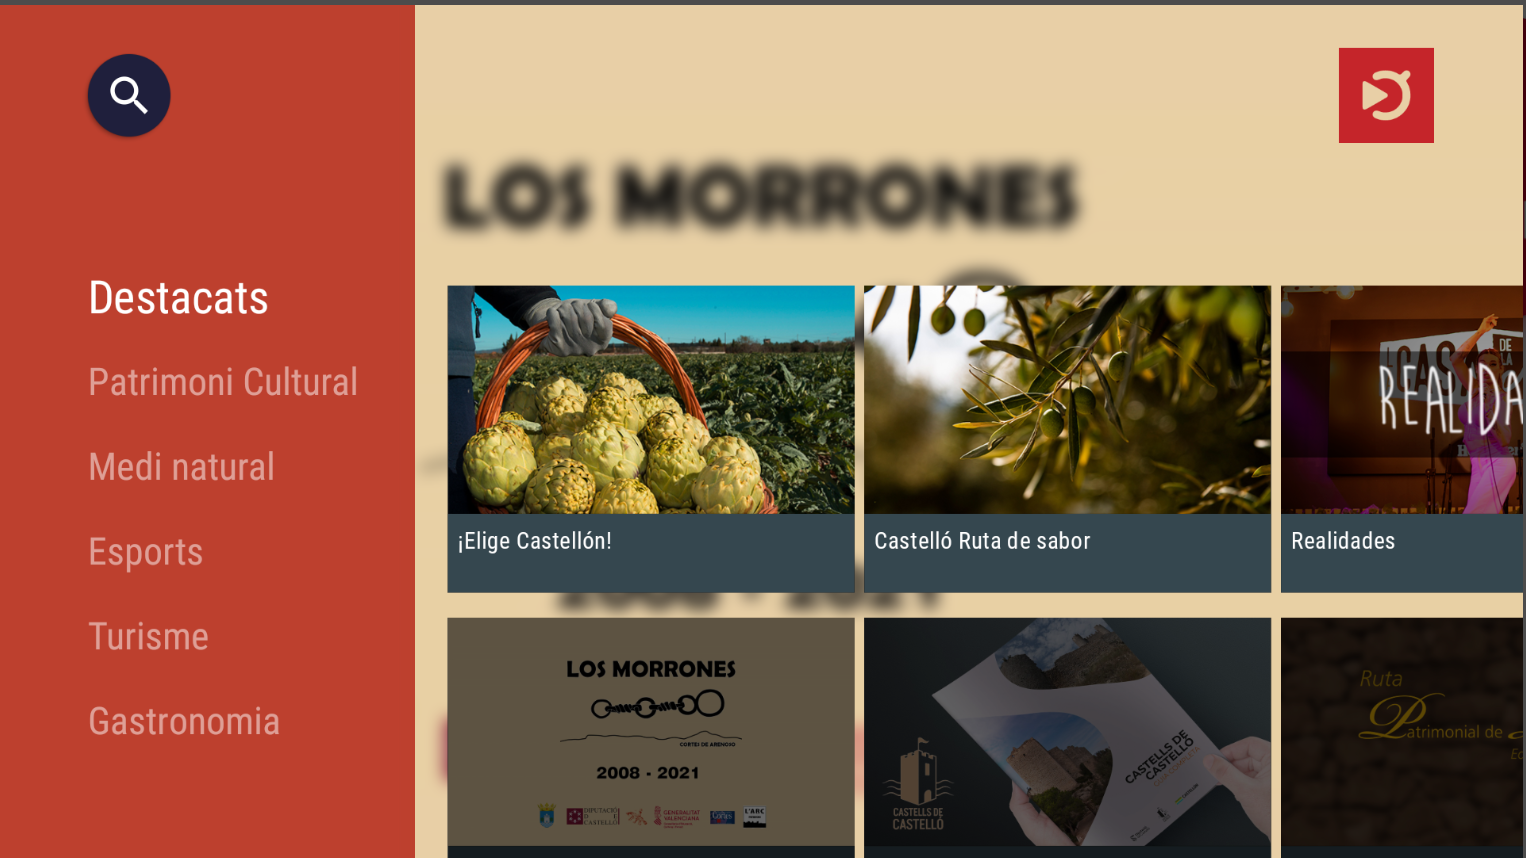
\includegraphics[width=0.8\textwidth]{imaxes/UX_inicios.png}
    \caption{Captura de la interfaz en las primeras fases del proyecto}
    \label{fig:UX_inicios}
\end{figure}
\begin{figure}[H]
    \centering
    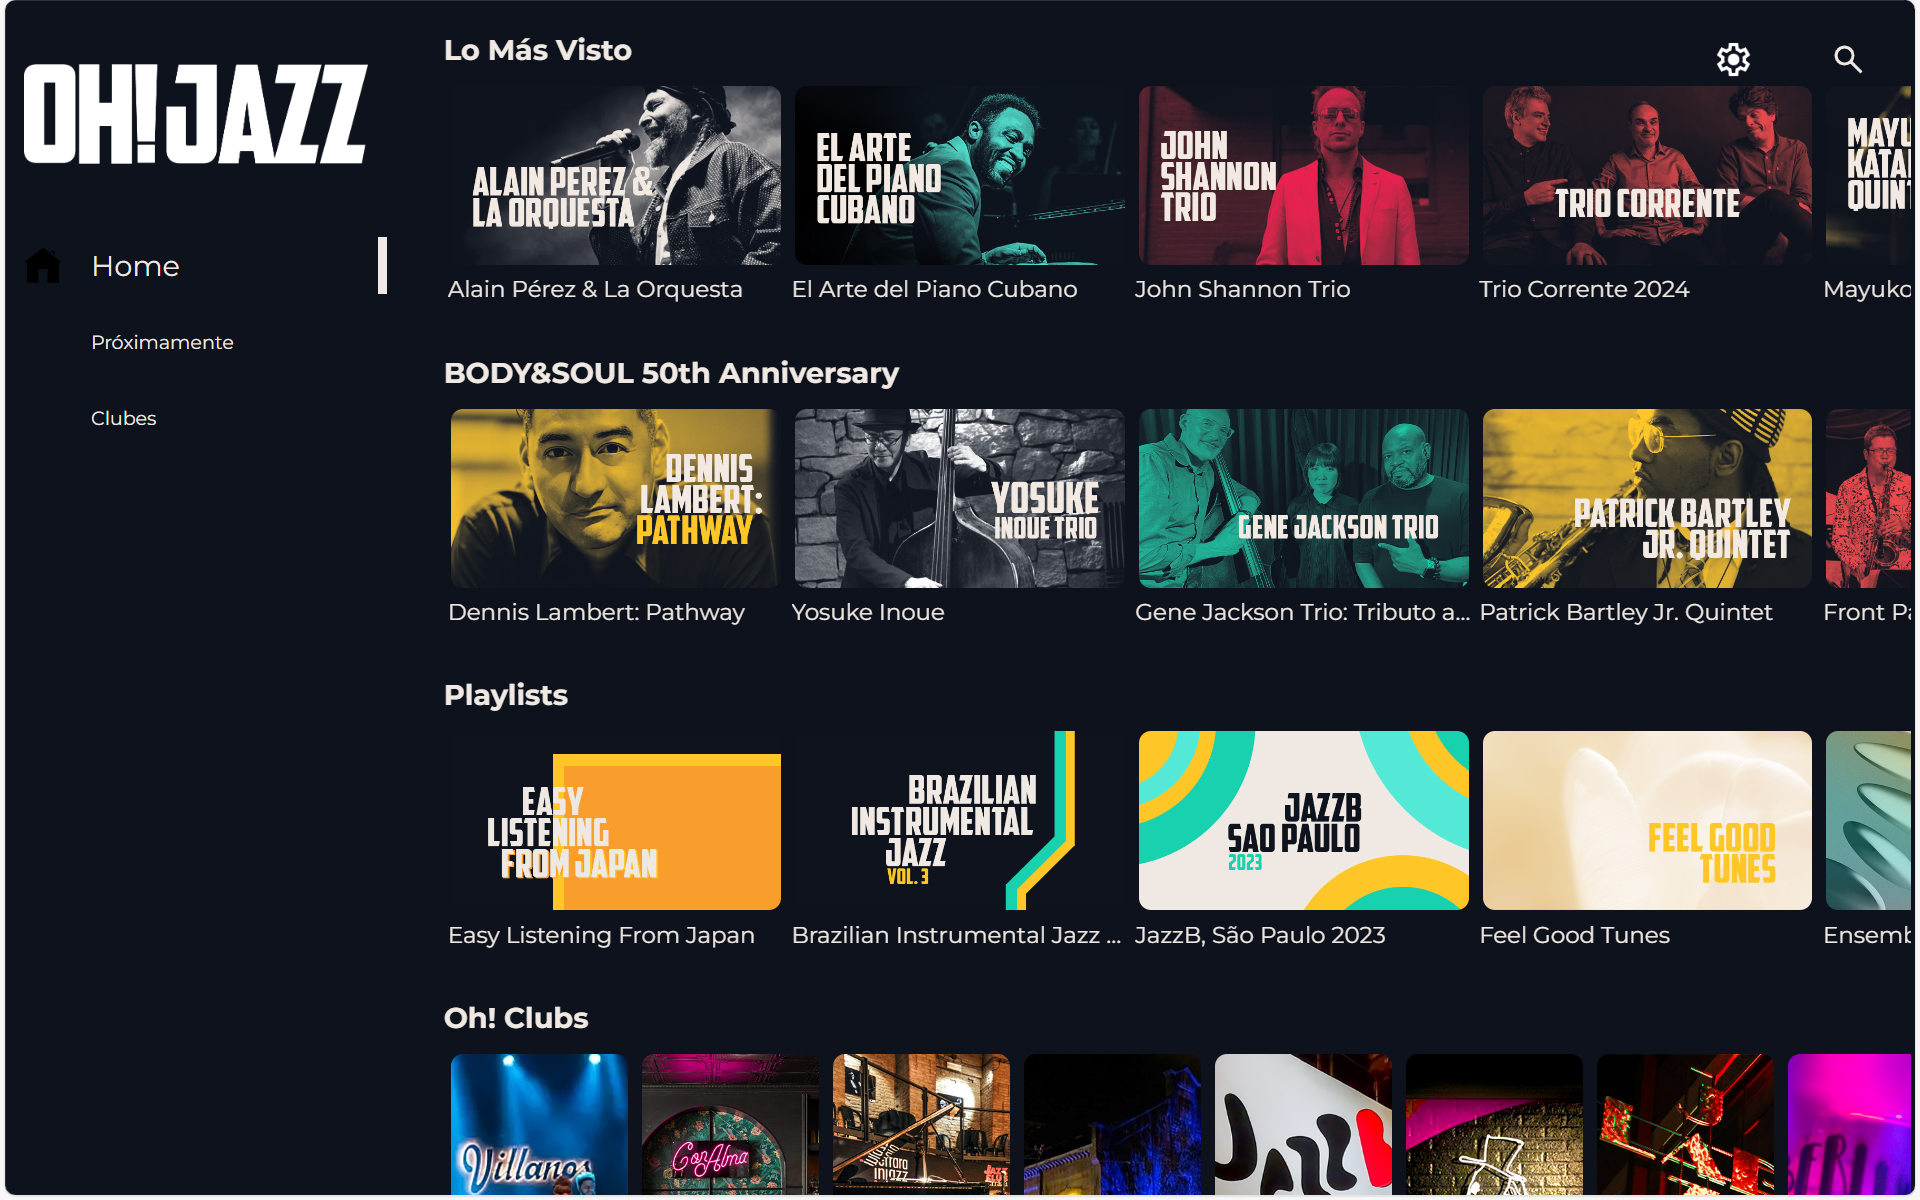
\includegraphics[width=0.8\textwidth]{imaxes/Home_desp_OhJazz.png}
    \caption{Captura de la interfaz más reciente, aún en pruebas por parte del cliente}
    \label{fig:Home_desp_OhJazz}
\end{figure}
\begin{figure}[H]
    \centering
    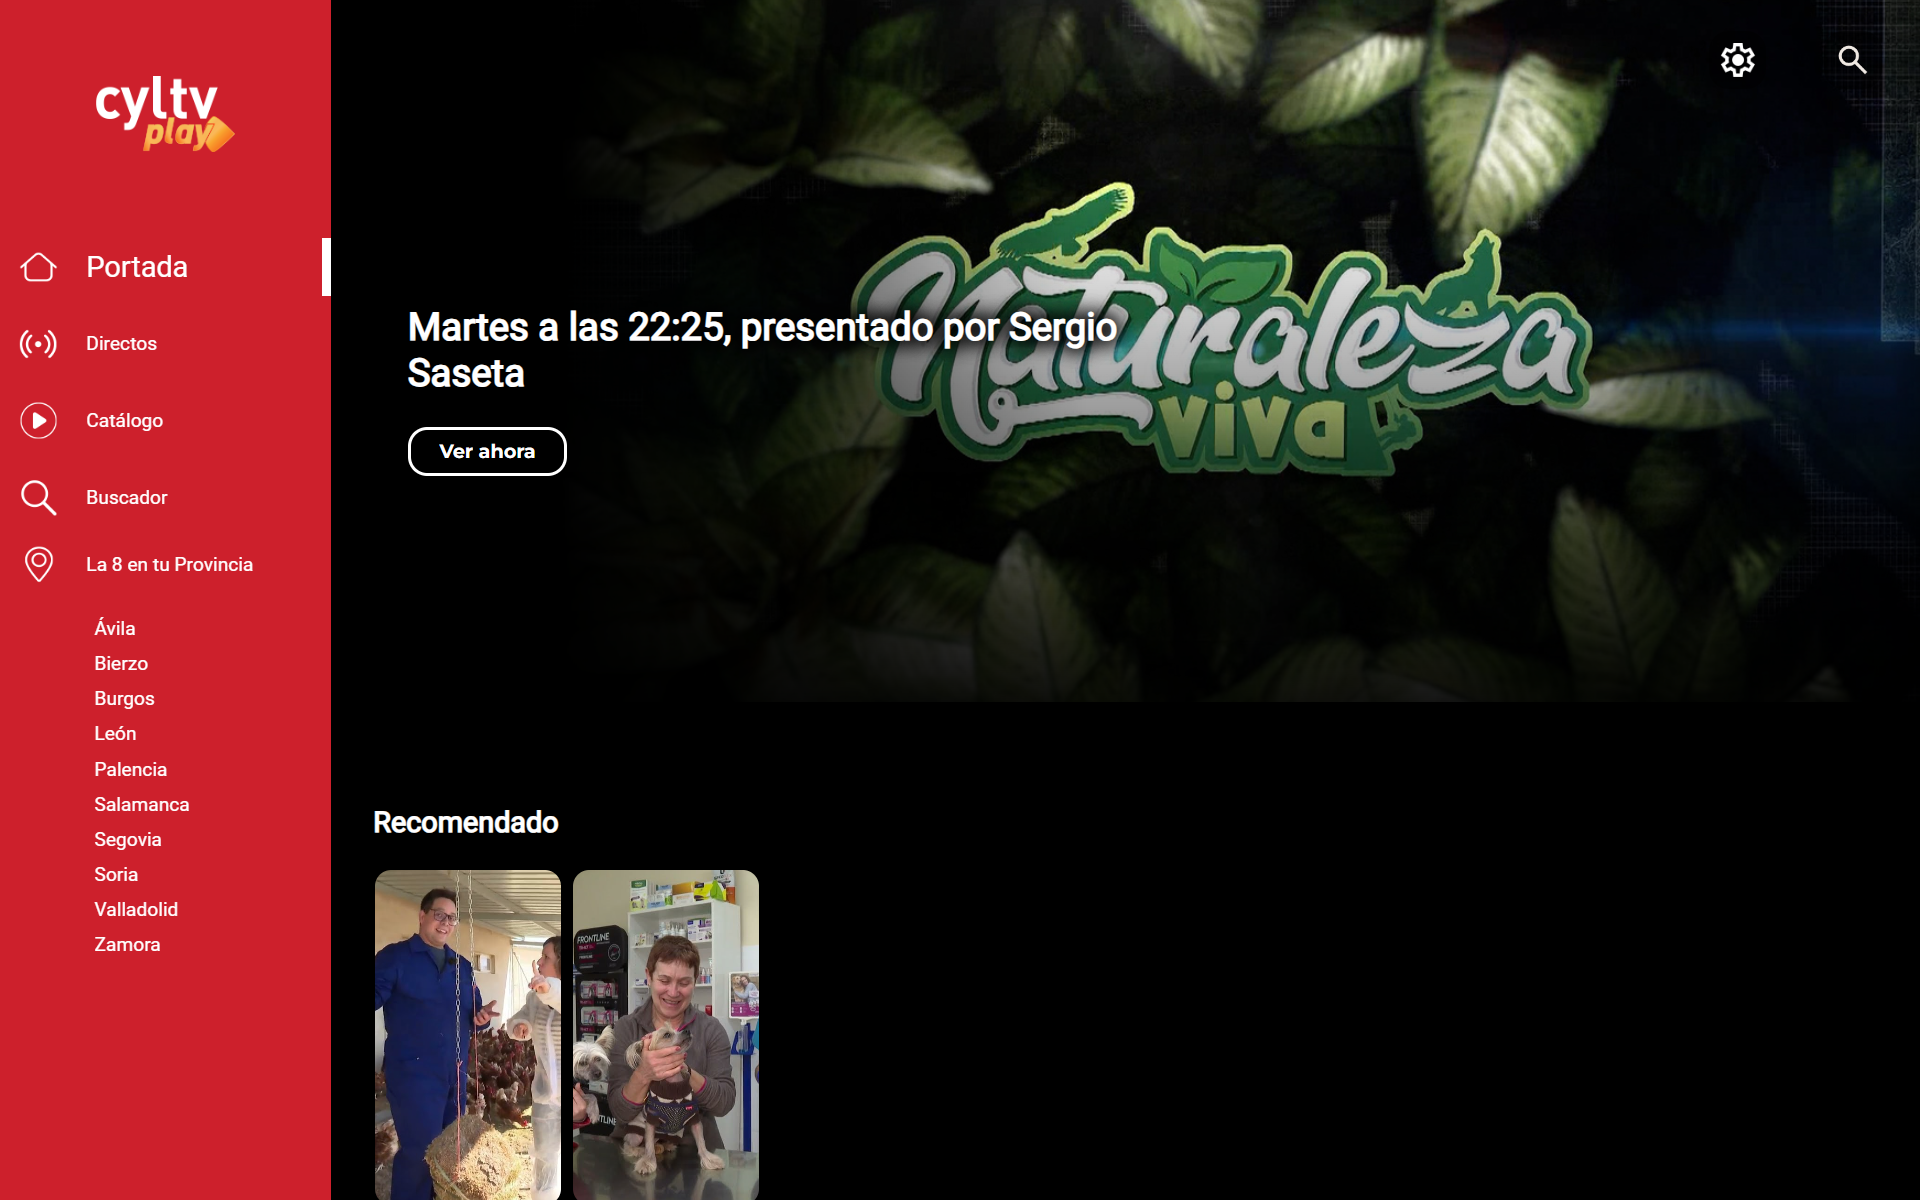
\includegraphics[width=0.8\textwidth]{imaxes/Home_CyLTv.png}
    \caption{Captura de la interfaz casi final}
    \label{fig:Home_CyLTv}
\end{figure}

Estas imágenes muestran la evolución de la interfaz de usuario de \textit{Ott}. La primera imagen refleja el diseño básico inicial, 
sin apenas funcionalidades. En la segunda, se observa un diseño más avanzado, aunque el cliente aún estaba ajustando parámetros (por ejemplo, 
la falta de visibilidad de los iconos de los menús o el contraste del fondo). Finalmente, la tercera imagen muestra la interfaz casi 
final, con un diseño pulido y todas las funcionalidades implementadas.

Más que enfocarse en un diseño único, el proyecto se ha centrado en el diseño de componentes y sus variantes. Algunos elementos de 
la interfaz tienen una estructura fija, aunque permiten personalizar colores y textos:

\begin{itemize}
    \item \textbf{Menú lateral:} Permite navegar por las secciones de la aplicación y se encuentra a la izquierda de la pantalla.
    \item \textbf{Menú superior:} Proporciona acceso a las opciones de configuración. Los iconos y colores de fondo son personalizables, pero la posición depende del número de opciones del menú.
    \item \textbf{Barra de búsqueda:} Situada en la pantalla de búsqueda, su posición y tamaño son fijos, pero utiliza los colores base del cliente para los efectos de foco y difuminado.
    \item \textbf{Lista de elementos:} Muestra los elementos disponibles en la aplicación. La estructura y tamaños son fijos, aunque el contenido y número de listas pueden personalizarse.
    \item \textbf{Detalle de elemento:} Muestra la información detallada de un elemento. Aunque la metadata y el contenido son personalizables, la estructura y disposición de los elementos son fijos. Se está trabajando para permitir mayor personalización desde el gestor de contenidos.
\end{itemize}

El cliente puede personalizar la interfaz ajustando colores de fondo, texto, botones, foco y añadiendo sus logos e imágenes, adaptando la 
aplicación a su identidad visual.
\subsubsection{Personalización de los componentes}
\label{sec:diseno-ux-personalizacion}

Como se ha mencionado anteriormente, el diseño de la interfaz de usuario se ha centrado en la creación de componentes y sus múltiples variantes. 
Estos componentes se dividen en dos tipos principales: \textit{contenidos} y \textit{contenedores}, cada uno de los cuales tiene un enfoque de 
diseño diferente dependiendo del tipo de \textit{widget} en el que se utilicen. Un \textit{widget} es un componente de la interfaz que almacena y 
muestra uno o varios contenidos de manera específica.

Cada tipo de \textit{widget} determina la presentación tanto de los contenidos como de los contenedores, lo que implica que se necesita un diseño y 
un código específico para asegurar que se muestren correctamente en la interfaz. A continuación, se detallan los aspectos clave que cambian según 
el tipo de \textit{widget}:

\begin{itemize}
    \item \textbf{Disposición de los contenidos:} Según el tipo de \textit{widget}, los contenidos se distribuyen de formas diversas. Si se trata de 
    un \textit{widget} de \textbf{destacados}, los contenidos se mostrarán con un tamaño más grande y ocuparán la parte superior de la pantalla, 
    siendo más llamativos. Estos \textit{widgets} pueden tener distintas configuraciones, como la inclusión de botones, un único contenido 
    destacado o varios en formato \textit{slider}, con opciones de distribución de texto e iconos. En contraste, un \textbf{mosaico} organizará los 
    contenidos de manera compacta en el centro de la pantalla. Para otros tipos de \textit{widgets}, como las listas horizontales, los contenidos 
    se dispondrán en filas secuenciales. Estos formatos son personalizables según las necesidades del cliente y el tipo de contenido que se desee resaltar.
    
    \item \textbf{Disposición de la información:} La cantidad y el tipo de información que se muestra también dependen del \textit{widget}. Por ejemplo, 
    en un \textbf{destacado}, el sistema puede mostrar el título, una descripción detallada y un botón de acceso al contenido. En un \textbf{banner}, 
    solo se mostrará el título del contenido. Esta flexibilidad en la información permite que los \textit{widgets} se ajusten a diferentes escenarios 
    y preferencias del cliente, lo que es clave para mantener una interfaz adaptable y eficaz.
    
    \item \textbf{Forma de las imágenes:} La forma y el tamaño de las imágenes asociadas a los contenidos varían según el tipo de \textit{widget}. 
    En los \textbf{destacados}, las imágenes suelen ser grandes, ocupando una buena parte de la pantalla, y pueden cambiar la distribución de la 
    información según el caso específico. En los \textbf{banners}, las imágenes tienen una orientación horizontal con un ratio de 16:9, mientras 
    que en los \textbf{posters}, las imágenes son verticales, con un ratio de 9:16. En los \textbf{posters}, las imágenes aparecen en un panel 
    lateral cuando el foco se mantiene en el contenido durante más de un segundo. Este enfoque garantiza una presentación visual coherente que 
    varía según el tipo de contenido y el diseño del \textit{widget}.
    
    \item \textbf{Otras características:} Algunos \textit{widgets} permiten funcionalidades adicionales que dependen del tipo de contenido que se esté 
    presentando. Por ejemplo, en los \textit{widgets} para contenidos en directo, puede aparecer una barra de progreso y el nombre del programa actual. 
    En un \textbf{widget banner-click}, diseñado para mostrar anuncios, se presenta un banner horizontal que ocupa casi todo el ancho de la pantalla, 
    y al hacer clic en él (excepto en televisores, donde esta opción está desactivada), redirige al usuario a una URL externa.
\end{itemize}

Estas personalizaciones, junto con otras más específicas o en desarrollo, deben estar correctamente implementadas y soportadas por la aplicación 
para garantizar que los \textit{widgets} seleccionados por el cliente funcionen sin problemas y no interfieran con el resto de la interfaz.

Adicionalmente, es importante tener en cuenta ciertas limitaciones en la personalización. Solo puede haber un \textit{widget destacado} por 
pantalla, los \textit{widgets} tipo \textbf{mosaico} con muchos elementos pueden sobrecargar la interfaz, y los \textbf{posters} se utilizan generalmente 
para destacar ciertos contenidos, mostrando información detallada sobre estos.

\subsubsection{Ejemplos de personalización}
\label{sec:diseno-ux-ejemplos}

A continuación se muestran algunos ejemplos de personalización de los widgets de la interfaz de usuario de \textit{Ott}.


\begin{figure}[H]
    \begin{subfigure}[c]{0.5\textwidth}
        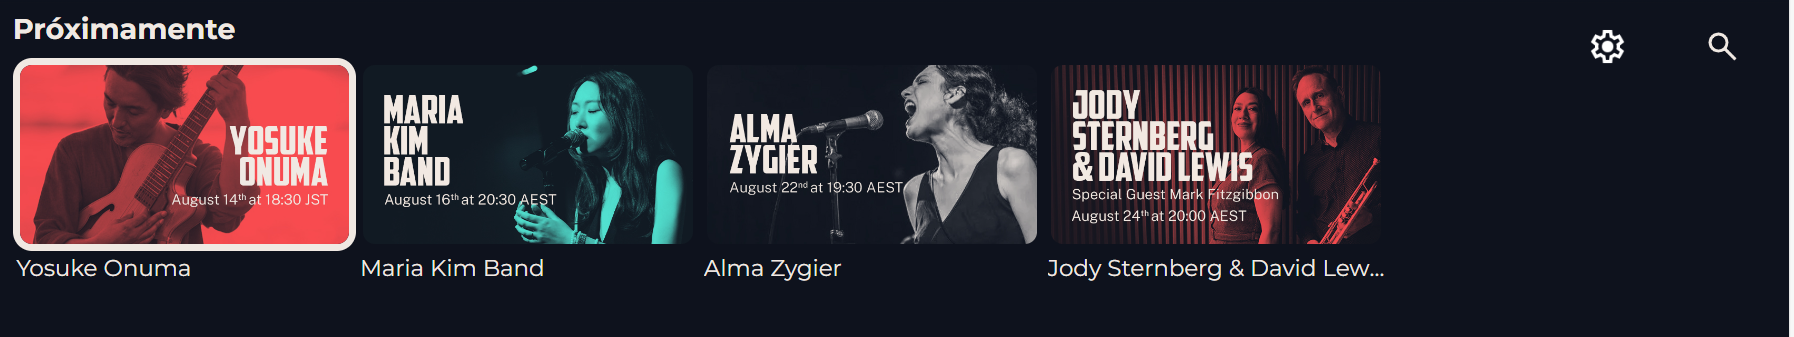
\includegraphics[width=\textwidth]{imaxes/Widget_banner.png}
        \subcaption{Ejemplo de un widget básico de tipo "banner"}
        \label{fig:Widget_banner}
    \end{subfigure}
    \hspace{0.1\textwidth}
    \begin{subfigure}[c]{0.5\textwidth}
        
\includegraphics[width=0.8\textwidth]{imaxes/Widget_destacado.png}
        \subcaption{Ejemplo de un widget básico de tipo "destacado"}
        \label{fig:Widget_destacado}
    \end{subfigure}
    \caption{Ejemplos de un widget básico de tipo "banner" y "destacado"}
    \label{fig:Widget_banner_destacado}
\end{figure}

\begin{figure}[H]
    \begin{subfigure}[c]{0.5\textwidth}
        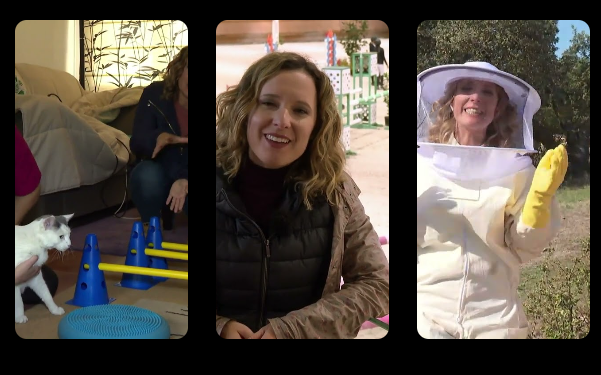
\includegraphics[width=\textwidth]{imaxes/Widget_poster.png}
        \subcaption{Ejemplo de un widget básico de tipo "poster"}
        \label{fig:Widget_poster}
    \end{subfigure}
    \hspace{0.1\textwidth}
    \begin{subfigure}[c]{0.5\textwidth}
        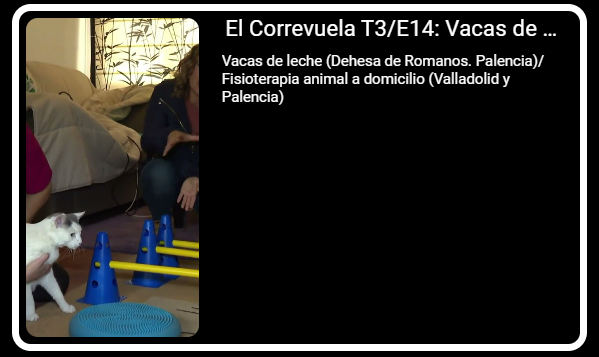
\includegraphics[width=\textwidth]{imaxes/Widget_poster_abierto.png}
        \subcaption{Ejemplo de un widget básico de tipo "poster" con la información mostrada}
        \label{fig:Widget_poster_abierto}
    \end{subfigure}
    \caption{Ejemplos de un widget básico de tipo "poster"}
    \label{fig:Widgets_poster}
\end{figure}

